\section{Condutor esférico. Campo uniforme}

\frame{
	\frametitle{Campo elétrico de um condutor esférico}
	\begin{block}{Introdução}
		Para um corpo de pequenas dimensões e carregado de eletricidade, desprezamos o seu volume e consideramos como se fosse uma carga elétrica concentrada num ponto. Nesse caso:
		$$E = K \ \dfrac{Q}{d^2}$$ \\
		\begin{itemize}
			\item Agora iremos estudar o caso onde iremos considerar uma esfera condutora eletrizada com carga elétrica $Q$ e de raio $R$.
		\end{itemize}
	\end{block}
}

\frame{
	\frametitle{Campo elétrico de um condutor esférico}
	\begin{block}{Introdução}
		\begin{itemize}
			\item Vamos supor que essa esfera esteja em equilíbrio eletrostático e afastada de qualquer outro corpo.
			\item Como a esfera encontra-se carregada, ela produz um campo elétrico à sua volta.
			\item Sendo assim, vamos determinar o valor do campo elétrico criado por essa esfera condutora eletrizada desde pontos infinitamente afastados até pontos internos.
		\end{itemize}
	\end{block}
}

\setmyunit{1cm}

\frame{
	\frametitle{Campo elétrico de um condutor esférico}
	\begin{block}{Possibilidades}
		Um ponto pode ocupar, relativamente à esfera, três posições: ou é \textbf{interno} (ponto A), ou \textbf{pertence} à esfera (ponto B), ou é \textbf{externo} (ponto C).
	\end{block}

	\vspace{0.3cm}
	
	\centering
	\scalebox{1}{

\tikzset{every picture/.style={line width=0.75pt}} %set default line width to 0.75pt        

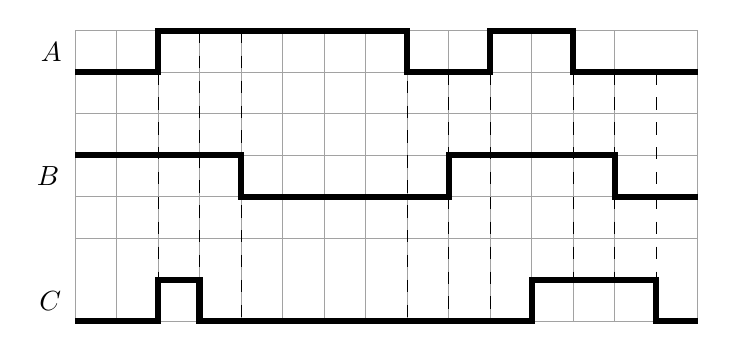
\begin{tikzpicture}[x=0.75pt,y=0.75pt,yscale=-1,xscale=1]
%uncomment if require: \path (0,300); %set diagram left start at 0, and has height of 300

%Shape: Grid [id:dp34531111101152123] 
\draw  [draw opacity=0] (100,40) -- (400,40) -- (400,180) -- (100,180) -- cycle ; \draw  [color={rgb, 255:red, 162; green, 162; blue, 162 }  ,draw opacity=1 ] (120,40) -- (120,180)(140,40) -- (140,180)(160,40) -- (160,180)(180,40) -- (180,180)(200,40) -- (200,180)(220,40) -- (220,180)(240,40) -- (240,180)(260,40) -- (260,180)(280,40) -- (280,180)(300,40) -- (300,180)(320,40) -- (320,180)(340,40) -- (340,180)(360,40) -- (360,180) ; \draw  [color={rgb, 255:red, 162; green, 162; blue, 162 }  ,draw opacity=1 ] (100,60) -- (400,60)(100,80) -- (400,80)(100,100) -- (400,100)(100,120) -- (400,120)(100,140) -- (400,140) ; \draw  [color={rgb, 255:red, 162; green, 162; blue, 162 }  ,draw opacity=1 ] (100,40) -- (400,40) -- (400,180) -- (100,180) -- cycle ;
%Straight Lines [id:da9908667716444586] 
\draw  [dash pattern={on 4.5pt off 4.5pt}]  (140,60) -- (140,160) ;


%Straight Lines [id:da9489034074703155] 
\draw  [dash pattern={on 4.5pt off 4.5pt}]  (160,40) -- (160,160) ;


%Straight Lines [id:da7444148673969375] 
\draw  [dash pattern={on 4.5pt off 4.5pt}]  (180,40) -- (180,180) ;


%Straight Lines [id:da33359589579811755] 
\draw  [dash pattern={on 4.5pt off 4.5pt}]  (260,40) -- (260,180) ;


%Straight Lines [id:da1689198722872045] 
\draw  [dash pattern={on 4.5pt off 4.5pt}]  (280,60) -- (280,180) ;


%Straight Lines [id:da2835936693187402] 
\draw  [dash pattern={on 4.5pt off 4.5pt}]  (300,60) -- (300,180) ;


%Straight Lines [id:da7069604701418795] 
\draw  [dash pattern={on 4.5pt off 4.5pt}]  (340,60) -- (340,160) ;


%Straight Lines [id:da35256438922338873] 
\draw  [dash pattern={on 4.5pt off 4.5pt}]  (360,60) -- (360,160) ;


%Straight Lines [id:da8396949759627998] 
\draw  [dash pattern={on 4.5pt off 4.5pt}]  (380,60) -- (380,160) ;


%Straight Lines [id:da8850959184881091] 
\draw [line width=2.25]    (100,60) -- (140,60) -- (140,40) -- (260,40) -- (260,60) -- (300,60) -- (300,40) -- (340,40) -- (340,60) -- (400,60) ;


%Straight Lines [id:da2574956876601695] 
\draw [line width=2.25]    (100,180) -- (140,180) -- (140,160) -- (160,160) -- (160,180) -- (320,180) -- (320,160) -- (380,160) -- (380,180) -- (400,180) ;


%Straight Lines [id:da8609754683162194] 
\draw [line width=2.25]    (100,100) -- (180,100) -- (180,120) -- (280,120) -- (280,100) -- (360,100) -- (360,120) -- (400,120) ;



% Text Node
\draw (88.5,50) node   {$A$};
% Text Node
\draw (87,110) node   {$B$};
% Text Node
\draw (88,170) node   {$C$};


\end{tikzpicture}
}
%	\centerline{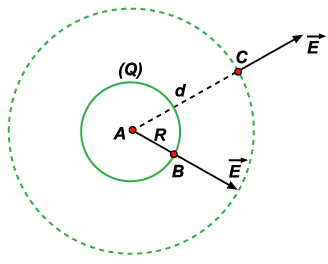
\includegraphics[width=0.45\linewidth]{Figuras/Ch08/condutor.png}}
}

\frame{
	\frametitle{Campo elétrico de um condutor esférico}
	\begin{block}{Caso $\#$01: ponto $A$ interno}
		A intensidade do vetor campo elétrico no interior de um condutor carregado de eletricidade e em equilíbrio eletrostático é sempre \textbf{nulo}.
	\end{block}
	
	\vspace{0.3cm}
	
	\centering
	\scalebox{1}{

\tikzset{every picture/.style={line width=0.75pt}} %set default line width to 0.75pt        

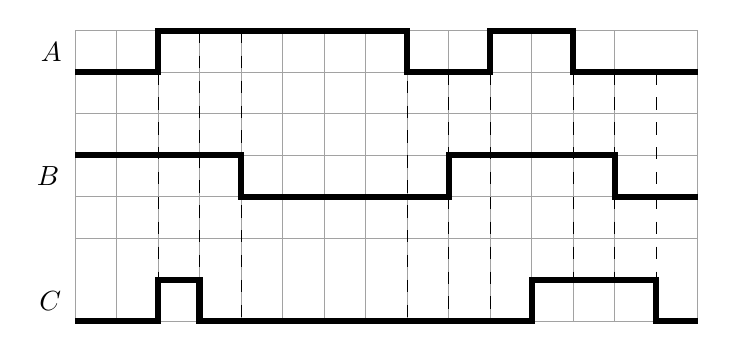
\begin{tikzpicture}[x=0.75pt,y=0.75pt,yscale=-1,xscale=1]
%uncomment if require: \path (0,300); %set diagram left start at 0, and has height of 300

%Shape: Grid [id:dp34531111101152123] 
\draw  [draw opacity=0] (100,40) -- (400,40) -- (400,180) -- (100,180) -- cycle ; \draw  [color={rgb, 255:red, 162; green, 162; blue, 162 }  ,draw opacity=1 ] (120,40) -- (120,180)(140,40) -- (140,180)(160,40) -- (160,180)(180,40) -- (180,180)(200,40) -- (200,180)(220,40) -- (220,180)(240,40) -- (240,180)(260,40) -- (260,180)(280,40) -- (280,180)(300,40) -- (300,180)(320,40) -- (320,180)(340,40) -- (340,180)(360,40) -- (360,180) ; \draw  [color={rgb, 255:red, 162; green, 162; blue, 162 }  ,draw opacity=1 ] (100,60) -- (400,60)(100,80) -- (400,80)(100,100) -- (400,100)(100,120) -- (400,120)(100,140) -- (400,140) ; \draw  [color={rgb, 255:red, 162; green, 162; blue, 162 }  ,draw opacity=1 ] (100,40) -- (400,40) -- (400,180) -- (100,180) -- cycle ;
%Straight Lines [id:da9908667716444586] 
\draw  [dash pattern={on 4.5pt off 4.5pt}]  (140,60) -- (140,160) ;


%Straight Lines [id:da9489034074703155] 
\draw  [dash pattern={on 4.5pt off 4.5pt}]  (160,40) -- (160,160) ;


%Straight Lines [id:da7444148673969375] 
\draw  [dash pattern={on 4.5pt off 4.5pt}]  (180,40) -- (180,180) ;


%Straight Lines [id:da33359589579811755] 
\draw  [dash pattern={on 4.5pt off 4.5pt}]  (260,40) -- (260,180) ;


%Straight Lines [id:da1689198722872045] 
\draw  [dash pattern={on 4.5pt off 4.5pt}]  (280,60) -- (280,180) ;


%Straight Lines [id:da2835936693187402] 
\draw  [dash pattern={on 4.5pt off 4.5pt}]  (300,60) -- (300,180) ;


%Straight Lines [id:da7069604701418795] 
\draw  [dash pattern={on 4.5pt off 4.5pt}]  (340,60) -- (340,160) ;


%Straight Lines [id:da35256438922338873] 
\draw  [dash pattern={on 4.5pt off 4.5pt}]  (360,60) -- (360,160) ;


%Straight Lines [id:da8396949759627998] 
\draw  [dash pattern={on 4.5pt off 4.5pt}]  (380,60) -- (380,160) ;


%Straight Lines [id:da8850959184881091] 
\draw [line width=2.25]    (100,60) -- (140,60) -- (140,40) -- (260,40) -- (260,60) -- (300,60) -- (300,40) -- (340,40) -- (340,60) -- (400,60) ;


%Straight Lines [id:da2574956876601695] 
\draw [line width=2.25]    (100,180) -- (140,180) -- (140,160) -- (160,160) -- (160,180) -- (320,180) -- (320,160) -- (380,160) -- (380,180) -- (400,180) ;


%Straight Lines [id:da8609754683162194] 
\draw [line width=2.25]    (100,100) -- (180,100) -- (180,120) -- (280,120) -- (280,100) -- (360,100) -- (360,120) -- (400,120) ;



% Text Node
\draw (88.5,50) node   {$A$};
% Text Node
\draw (87,110) node   {$B$};
% Text Node
\draw (88,170) node   {$C$};


\end{tikzpicture}
}
%	\centerline{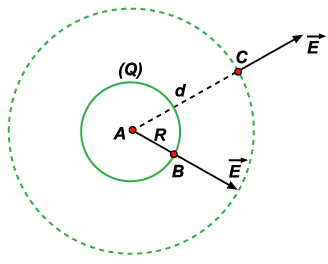
\includegraphics[width=0.45\linewidth]{Figuras/Ch08/condutor.png}}
}

\frame{
	\frametitle{Campo elétrico de um condutor esférico}
	\begin{block}{Caso $\#$02: ponto $B$ pertencente à esfera}
		Dependendo do modelo adotado para a distribuição de carga a resposta é diferente. Em livros razoáveis de ensino médio e mesmo em livros de Física Geral de ensino superior o assunto é convenientemente evitado pelos autores.
		\begin{itemize}
			\item Este tema não é adequado ao ensino médio.
		\end{itemize}
	\end{block}

%	\vspace{0.3cm}
	
	\centering
	\scalebox{1}{

\tikzset{every picture/.style={line width=0.75pt}} %set default line width to 0.75pt        

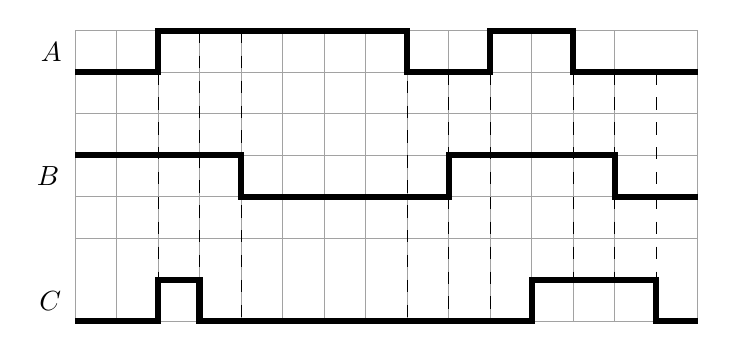
\begin{tikzpicture}[x=0.75pt,y=0.75pt,yscale=-1,xscale=1]
%uncomment if require: \path (0,300); %set diagram left start at 0, and has height of 300

%Shape: Grid [id:dp34531111101152123] 
\draw  [draw opacity=0] (100,40) -- (400,40) -- (400,180) -- (100,180) -- cycle ; \draw  [color={rgb, 255:red, 162; green, 162; blue, 162 }  ,draw opacity=1 ] (120,40) -- (120,180)(140,40) -- (140,180)(160,40) -- (160,180)(180,40) -- (180,180)(200,40) -- (200,180)(220,40) -- (220,180)(240,40) -- (240,180)(260,40) -- (260,180)(280,40) -- (280,180)(300,40) -- (300,180)(320,40) -- (320,180)(340,40) -- (340,180)(360,40) -- (360,180) ; \draw  [color={rgb, 255:red, 162; green, 162; blue, 162 }  ,draw opacity=1 ] (100,60) -- (400,60)(100,80) -- (400,80)(100,100) -- (400,100)(100,120) -- (400,120)(100,140) -- (400,140) ; \draw  [color={rgb, 255:red, 162; green, 162; blue, 162 }  ,draw opacity=1 ] (100,40) -- (400,40) -- (400,180) -- (100,180) -- cycle ;
%Straight Lines [id:da9908667716444586] 
\draw  [dash pattern={on 4.5pt off 4.5pt}]  (140,60) -- (140,160) ;


%Straight Lines [id:da9489034074703155] 
\draw  [dash pattern={on 4.5pt off 4.5pt}]  (160,40) -- (160,160) ;


%Straight Lines [id:da7444148673969375] 
\draw  [dash pattern={on 4.5pt off 4.5pt}]  (180,40) -- (180,180) ;


%Straight Lines [id:da33359589579811755] 
\draw  [dash pattern={on 4.5pt off 4.5pt}]  (260,40) -- (260,180) ;


%Straight Lines [id:da1689198722872045] 
\draw  [dash pattern={on 4.5pt off 4.5pt}]  (280,60) -- (280,180) ;


%Straight Lines [id:da2835936693187402] 
\draw  [dash pattern={on 4.5pt off 4.5pt}]  (300,60) -- (300,180) ;


%Straight Lines [id:da7069604701418795] 
\draw  [dash pattern={on 4.5pt off 4.5pt}]  (340,60) -- (340,160) ;


%Straight Lines [id:da35256438922338873] 
\draw  [dash pattern={on 4.5pt off 4.5pt}]  (360,60) -- (360,160) ;


%Straight Lines [id:da8396949759627998] 
\draw  [dash pattern={on 4.5pt off 4.5pt}]  (380,60) -- (380,160) ;


%Straight Lines [id:da8850959184881091] 
\draw [line width=2.25]    (100,60) -- (140,60) -- (140,40) -- (260,40) -- (260,60) -- (300,60) -- (300,40) -- (340,40) -- (340,60) -- (400,60) ;


%Straight Lines [id:da2574956876601695] 
\draw [line width=2.25]    (100,180) -- (140,180) -- (140,160) -- (160,160) -- (160,180) -- (320,180) -- (320,160) -- (380,160) -- (380,180) -- (400,180) ;


%Straight Lines [id:da8609754683162194] 
\draw [line width=2.25]    (100,100) -- (180,100) -- (180,120) -- (280,120) -- (280,100) -- (360,100) -- (360,120) -- (400,120) ;



% Text Node
\draw (88.5,50) node   {$A$};
% Text Node
\draw (87,110) node   {$B$};
% Text Node
\draw (88,170) node   {$C$};


\end{tikzpicture}
}
}

\frame{
	\frametitle{Campo elétrico de um condutor esférico}
	\begin{block}{Caso $\#$03: ponto $C$ externo}
		O campo produzido num ponto externo de uma esfera pode ser calculado admitindo-se que a carga da esfera seja \textbf{puntiforme} e colocada no \textbf{centro da esfera}, em vez de estar distribuída pela superfície.
		$$E = K \ \dfrac{Q}{d^2}$$
	\end{block}
	
%	\vspace{0.3cm}
	
	\centering
	\scalebox{1}{

\tikzset{every picture/.style={line width=0.75pt}} %set default line width to 0.75pt        

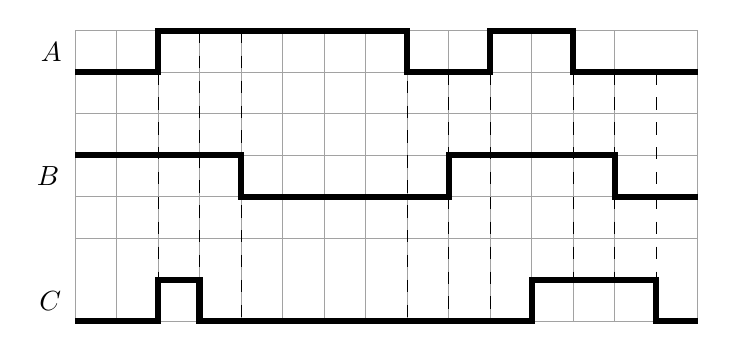
\begin{tikzpicture}[x=0.75pt,y=0.75pt,yscale=-1,xscale=1]
%uncomment if require: \path (0,300); %set diagram left start at 0, and has height of 300

%Shape: Grid [id:dp34531111101152123] 
\draw  [draw opacity=0] (100,40) -- (400,40) -- (400,180) -- (100,180) -- cycle ; \draw  [color={rgb, 255:red, 162; green, 162; blue, 162 }  ,draw opacity=1 ] (120,40) -- (120,180)(140,40) -- (140,180)(160,40) -- (160,180)(180,40) -- (180,180)(200,40) -- (200,180)(220,40) -- (220,180)(240,40) -- (240,180)(260,40) -- (260,180)(280,40) -- (280,180)(300,40) -- (300,180)(320,40) -- (320,180)(340,40) -- (340,180)(360,40) -- (360,180) ; \draw  [color={rgb, 255:red, 162; green, 162; blue, 162 }  ,draw opacity=1 ] (100,60) -- (400,60)(100,80) -- (400,80)(100,100) -- (400,100)(100,120) -- (400,120)(100,140) -- (400,140) ; \draw  [color={rgb, 255:red, 162; green, 162; blue, 162 }  ,draw opacity=1 ] (100,40) -- (400,40) -- (400,180) -- (100,180) -- cycle ;
%Straight Lines [id:da9908667716444586] 
\draw  [dash pattern={on 4.5pt off 4.5pt}]  (140,60) -- (140,160) ;


%Straight Lines [id:da9489034074703155] 
\draw  [dash pattern={on 4.5pt off 4.5pt}]  (160,40) -- (160,160) ;


%Straight Lines [id:da7444148673969375] 
\draw  [dash pattern={on 4.5pt off 4.5pt}]  (180,40) -- (180,180) ;


%Straight Lines [id:da33359589579811755] 
\draw  [dash pattern={on 4.5pt off 4.5pt}]  (260,40) -- (260,180) ;


%Straight Lines [id:da1689198722872045] 
\draw  [dash pattern={on 4.5pt off 4.5pt}]  (280,60) -- (280,180) ;


%Straight Lines [id:da2835936693187402] 
\draw  [dash pattern={on 4.5pt off 4.5pt}]  (300,60) -- (300,180) ;


%Straight Lines [id:da7069604701418795] 
\draw  [dash pattern={on 4.5pt off 4.5pt}]  (340,60) -- (340,160) ;


%Straight Lines [id:da35256438922338873] 
\draw  [dash pattern={on 4.5pt off 4.5pt}]  (360,60) -- (360,160) ;


%Straight Lines [id:da8396949759627998] 
\draw  [dash pattern={on 4.5pt off 4.5pt}]  (380,60) -- (380,160) ;


%Straight Lines [id:da8850959184881091] 
\draw [line width=2.25]    (100,60) -- (140,60) -- (140,40) -- (260,40) -- (260,60) -- (300,60) -- (300,40) -- (340,40) -- (340,60) -- (400,60) ;


%Straight Lines [id:da2574956876601695] 
\draw [line width=2.25]    (100,180) -- (140,180) -- (140,160) -- (160,160) -- (160,180) -- (320,180) -- (320,160) -- (380,160) -- (380,180) -- (400,180) ;


%Straight Lines [id:da8609754683162194] 
\draw [line width=2.25]    (100,100) -- (180,100) -- (180,120) -- (280,120) -- (280,100) -- (360,100) -- (360,120) -- (400,120) ;



% Text Node
\draw (88.5,50) node   {$A$};
% Text Node
\draw (87,110) node   {$B$};
% Text Node
\draw (88,170) node   {$C$};


\end{tikzpicture}
}
}

\frame{
	\frametitle{Campo elétrico de um condutor esférico}
	\begin{block}{Exemplo \#01}
		Uma esfera condutora de raio $R = \SI{40}{\centi\meter}$ está eletrizada uniformemente com carga $Q = \SI{4.0}{\micro\coulomb}$. (a) Determine a intensidade do campo elétrico num ponto $P$ à \SI{60}{\centi\meter} da superfície da esfera. (b) Qual o valor da força sobre uma carga de prova $q = \SI{2.0}{\micro\coulomb}$ colocada no ponto $P$?
	\end{block}
}

\frame{
	\frametitle{Campo elétrico de um condutor esférico}
	\begin{block}{Resolução}
		(a) A distância total a ser considerada é de $40 + 60 = \SI{100}{\centi\meter}$ = \SI{1}{\meter}. Então:
		
		\[ E = K \ \dfrac{Q}{d^2} = \num{9e9} \ \dfrac{\num{4,0e-6}}{1^2} = \SI{3.6e4}{\newton\per\coulomb} \]
		
		(b) $F = q \times E = \num{2,0e-6}\cdot \num{3.6e4} = \SI{7.2e-2}{\newton}$.
	\end{block}
}

\frame{
	\frametitle{Linhas de força}
	\begin{block}{Definição}
		São a \textbf{representação geométrica} convencionada para \textbf{indicar a presença de campos elétricos}, sendo representadas por linhas  que tangenciam os vetores campo elétrico resultante em cada ponto. Por convenção, as linhas de força têm a mesma orientação do vetor campo elétrico, de modo que para campos gerados por cargas positivas as linhas de força são \textbf{divergentes} (sentido de afastamento) e campos gerados por cargas elétricas negativas são representados por linhas de força \textbf{convergentes} (sentido de aproximação).
	\end{block}
}

\frame{
	\frametitle{Linhas de força}
	\begin{block}{Propriedade $\#$01}
		Quando se trabalha com cargas geradoras sem dimensões (cargas pontuais), as linhas de força são sempre abertas, ou seja, não se fecham sobre si. Elas sempre \textbf{“saem” das cargas positivas} e \textbf{“entram” nas cargas de sinal negativo}.
	\end{block}

	\setmyunit{1cm}

	\begin{minipage}{0.49\linewidth}
		\centering
		\begin{tikzpicture}
			\foreach \x in {0,22.5,...,337.5} {
				\draw[-Latex,blue] (0,0) -- (\x:2);
			}
			
			\filldraw[fill=white,draw=black] (0,0) circle (0.5) node {$ + $};
		\end{tikzpicture}
	\end{minipage}
	\hfill
	\begin{minipage}{0.49\linewidth}
		\centering
		\begin{tikzpicture}
		\foreach \x in {0,22.5,...,337.5} {
			\draw[blue] (0,0) -- (\x:2);
			\draw[-Latex,blue] (\x:2) -- (\x:1.5);
		}
		
		\filldraw[fill=white,draw=black] (0,0) circle (0.5) node {$ - $};
		\end{tikzpicture}
	\end{minipage}

	
%	\centerline{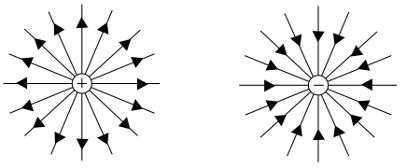
\includegraphics[width=0.8\linewidth]{Figuras/Ch08/linhas1.jpg}}
}

\frame{
	\frametitle{Linhas de força}
	\begin{block}{Propriedade $\#$02}
		As linhas de força nunca podem começar e terminar na mesma carga elétrica. Quanto \textbf{mais próximas} estiverem desenhadas as linhas de força em alguma região do espaço, \textbf{maior é o módulo do campo elétrico} naquela região.
	\end{block}
	\centerline{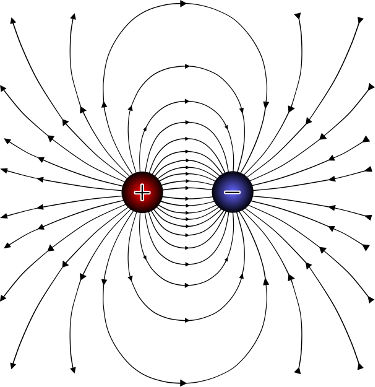
\includegraphics[width=0.4\linewidth]{Figuras/Ch08/linhas2.jpg}}
}

\frame{
	\frametitle{Linhas de força}
	\begin{block}{Propriedade $\#$03}
		Se o campo elétrico local for \textbf{nulo}, não haverá linhas de força na região.
	\end{block}
}

\frame{
	\frametitle{Linhas de força}
	\begin{block}{Propriedade $\#$04}
		A \textbf{tangente} de qualquer ponto em cima de uma linha de força indica a \textbf{direção do campo elétrico resultante}. Portanto, se uma carga de prova for colocada nesse ponto, ela sofrerá a ação de uma força elétrica na mesma direção.
	\end{block}
}

\frame{
	\frametitle{Linhas de força}
	\begin{block}{Propriedade $\#$05}
		Quando uma carga elétrica \textbf{move-se na direção de uma linha de força}, a força elétrica \textbf{realiza trabalho} sobre ela, transformando energia potencial elétrica em energia cinética ou vice-versa. Quando uma carga elétrica move-se em uma \textbf{direção perpendicular a uma linha de força}, a força elétrica \textbf{não realiza trabalho} sobre ela e, dessa forma, tanto a sua energia potencial elétrica quanto a sua energia cinética devem permanecer constantes.
	\end{block}
}

\frame{
	\frametitle{Linhas de força}
	\begin{block}{Propriedade $\#$06}
		Duas ou mais linhas de força \textbf{não se cruzam}, uma vez que elas já representam a soma vetorial dos campos elétricos naquele ponto do espaço.
	\end{block}
	\centerline{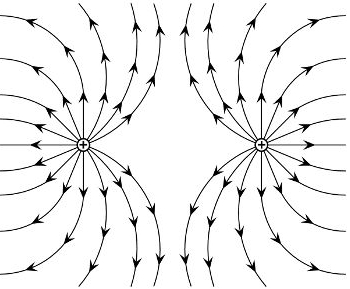
\includegraphics[width=0.5\linewidth]{Figuras/Ch08/linhas3.jpg}}
}

\frame{
	\frametitle{Campo elétrico uniforme}
	\begin{block}{Definição}
		Dizemos que um campo elétrico é uniforme em uma região quando suas \textbf{linhas de força são paralelas} e igualmente espaçadas umas das outras, o que implica que seu vetor campo elétrico nesta região tem, em todos os pontos, \textbf{mesma intensidade, direção e sentido}, isto é, $\vec{E}$ possui as mesmas características em todos os seus pontos.
	\end{block}
}

\frame{
	\frametitle{Campo elétrico uniforme}
	\begin{block}{Como obtê-lo?}
		Suponhamos dois condutores planos, paralelos e próximos. Se eles forem carregados com cargas de mesmo valor absoluto e sinais opostos, o campo elétrico que se formará entre eles será uniforme. As linhas de força são paralelas entre si e perpendiculares aos planos; apenas nos contornos o campo deixa de ser uniforme: as linhas de força se curvam.
	\end{block}

	\centering
	
	\medskip

	\newcommand{\innercolor}{gray!70!white}
	\newcommand{\outercolor}{gray!40!white}
	\newcommand{\leftcoil}{red!75!gray}
	\pgfmathsetmacro{\coilseparation}{0.02}
	
	\pgfmathsetmacro{\halflinewidth}{0.008}
	
	
	\begin{tikzpicture}[x={(\xx*1cm,\xy*1cm)},y={(\yx*1cm,\yy*1cm)},z={(\zx*1cm,\zy*1cm)}]
	\draw[\leftcoil, thick] (-0.02,5,1.125) -- +(0,2,0) (1.02,5,3.875) -- +(0,2,0);
	
	\draw[dashed,<->] ($ (-0.02,5,1.125)+(0,2,0) $) -- ($ (1.02,5,3.875)+(0,2,0) $);
	\node[rotate=85] at ($ (-0.02,5+2,1.125)!0.5!(1.02,5+2,3.875)+(0,0.2,0) $) {$ V_p $};
	
	\draw[-latex] (-0.02,6.5,1.325) -- node[above] {$ i_p $} +(0,-1,0);
	\draw[latex-] (1.02,0.02-0.5,1.3) -- node[above] {$ i_s $} +(0,-1,0);
	
	\filldraw[fill=\innercolor]  (0,1,1) -- (1,1,1) -- (1,4,1) -- (0,4,1) -- cycle;
	\filldraw[fill=\innercolor]  (1,4,1) -- (0,4,1) -- (0,4,4) -- (1,4,4) -- cycle;
	\filldraw[fill=\innercolor]  (0,0,0) -- (1,0,0) -- (1,0,5) -- (0,0,5) -- cycle;
	\filldraw[fill=\innercolor]  (0,0,5) -- (0,5,5) -- (1,5,5) -- (1,0,5) -- cycle;
	\filldraw[fill=\outercolor,even odd rule]    (0,0,0) -- (0,5,0) -- (0,5,5) -- (0,0,5) --cycle (0,1,1) -- (0,4,1) -- (0,4,4) -- (0,1,4) --cycle ;
	
	\begin{scope}
	\clip (0,3,1) -- (0,6,1) -- (0,6,4) -- (0,3,4);
	\foreach \z in {1.125,1.375,...,3.875}
	{   \draw[\leftcoil,thick] (0,5,\z) -- (-\coilseparation,5,\z) -- (-\coilseparation,4-\coilseparation,\z) -- (1+\coilseparation,4-\coilseparation,\z) -- (1+\coilseparation,4,\z);
	}
	\end{scope}
	
	
	\foreach \z in {1.25,1.75,...,3.75}
	{   \draw[blue,thick] (0,1,\z) -- (-\coilseparation,1,\z) -- (-\coilseparation,0-\coilseparation,\z) -- (1+\coilseparation,0-\coilseparation,\z) -- (1+\coilseparation,0,\z);
	}

	\draw[blue,thick] (1+\coilseparation,0+\coilseparation,1.1) -- +(0,-2,0) (-\coilseparation,1+\coilseparation,3.85) -- +(0,-3,0);
	
	\draw[dashed,<->] (1.02,-2+0.02,1.1) -- (-0.02,0.02-2,3.85);
	\node[rotate=-70] at ($ (1.02,-2+0.02,1.1)!0.5!(-0.02,0.02-2,3.85)+(0,-0.2,0) $) {$ V_s $};
	
	\draw[decorate,decoration={brace,amplitude=10pt},xshift=-4pt,yshift=0pt] (0,5,1.25) -- +(0,0,2.75);
	\draw[decorate,decoration={brace,amplitude=10pt},xshift=-4pt,yshift=0pt] (1.2,0,3.75) -- +(0,0,-2.6);
	\node[rotate=90] at (0,5.7,2.625) {$ N_p $ espiras};
	\node[rotate=-90] at (1.2,-0.5,2.5) {$ N_s $ espiras};
	
	\draw[dashed,postaction={decorate,decoration={markings,mark=between positions 0.1 and 1 step 0.2 with \arrow{Latex}}}] (0,4.5,0.5) -- (0,0.5,0.5) -- ++(0,0,4) -- ++(0,4,0) -- cycle;
	
	\draw[] (0,2.5,4.7)% -- +(0,-0.5,1.5)
	node[rotate=-10] {Fluxo magnético ($ \phi $)};
	
	\end{tikzpicture}
%	\centerline{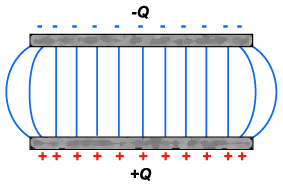
\includegraphics[width=0.5\linewidth]{Figuras/Ch08/uniforme1.png}}
}

\section*{Exercícios}

\frame{
	\frametitle{Exercícios}
	\begin{block}{}

		01. Num campo elétrico uniforme de intensidade $E = \SI{5.0e3}{\newton\per\coulomb}$ direção vertical e sentido de baixo para cima, é colocada em repouso uma partícula $q = \SI{2.0}{\micro\coulomb}$. Sendo $m = \SI{4.0}{\gram}$ a massa da partícula e desprezando as ações da gravidade, determine a aceleração adquirida pela partícula.

		\vspace{0.5cm}

		02. Considere uma esfera metálica de raio $R$, com uma carga elétrica $Q$ uniformemente distribuída em sua superfície. Num ponto $P$, a uma distância $2R$ do centro da esfera, o campo elétrico vale $E$. Determine o valor do	campo elétrico a uma distância $3R$ da superfície da esfera.
	\end{block}
}


\section*{Referências}

\frame{
	\frametitle{Referências e Exercícios Complementares}
	\begin{itemize}
		\item Física, Ciência e Tecnologia – Vol 3. PENTEADO, Paulo César M; TORRES, Carlos Magno A. Ed. Moderna (2006)
	\end{itemize}
	%\centering{\alert{Página 36 - \textbf{1.6.1 até 1.6.5, 1.6.17 até 1.6.19}}} \\
	%https://www.youtube.com/watch?v=IUgS7Uw-qBI
	\centering{\alert{Lista de exercícios 08}}
}